%%%%%%%%%%%%%%%%%%%%%%%%%%%%%%%%%%%%%%%%%%%%%%%%%%%%%%%%%%%%%%%%%%%%%%
% BeamerTemplate
% February 15, 2016
% By Simon David Pratt (mostly)

% remove aspectratio=169 if you want 4:3 ratio instead of 16:9
\documentclass[aspectratio=169]{beamer}
\usepackage{styles/presentation}

\title{Presentation Title}
\subtitle{Subtitle}

\author[Short Author List]{Long\\Author\\List}

\date{\today}

\newcommand{\bi}{\begin{itemize}}
\newcommand{\ei}{\end{itemize}}

\newcommand{\bn}{\begin{enumerate}}
\newcommand{\en}{\end{enumerate}}

%%% BEGIN DOCUMENT
\begin{document}

\frame[plain]{\titlepage}

\begin{frame}{Lists and Columns}
  \begin{columns}[T]
    \begin{column}{0.3\textwidth}
    \end{column}
    \begin{column}{0.4\textwidth}
      \bi
    \item Itemized lists are useful
      \bi
    \item Often with sub-lists
      \ei
      \bn
    \item Or enumerations\\(which assign a number to each item)
    \item If order is important
      \en
    \item Narrow columns are easier to read
      \ei
    \end{column}
    \begin{column}{0.3\textwidth}
    \end{column}
  \end{columns}
\end{frame}

\begin{frame}{Background: \texttt{malloc} and \texttt{mmap}}
  \begin{columns}[T]
    \begin{column}{0.5\textwidth}
      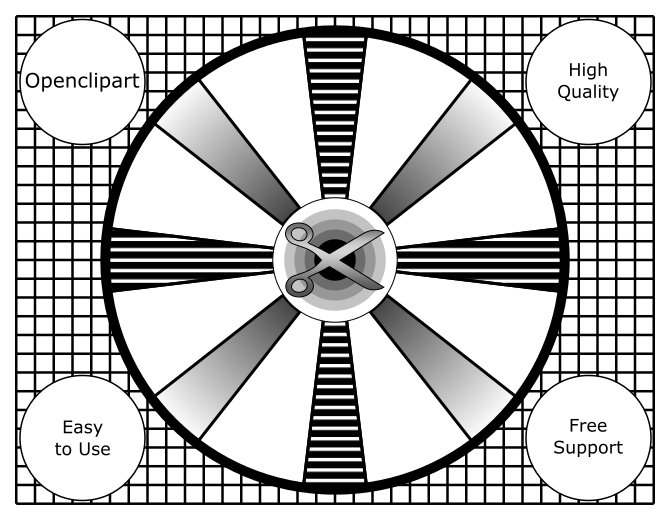
\includegraphics[scale=0.3]{./figures/Retro.png}
    \end{column}
    \begin{column}{0.5\textwidth}
      \bi
      \item Mixing text and images on slides is good
      \ei
    \end{column}
  \end{columns}
\end{frame}

\begin{frame}{tikz: Animated Diagrams}
  \begin{columns}[T]
    \begin{column}{0.1\textwidth}
        \vspace{2cm}
        \begin{tikzpicture}[node distance=1cm,overlay]
          \tikzstyle{every node}=[draw]
          % nodes
          \node<1-8> (M) {M};
          \node (T2) [below of=M] {$T_2$};
          \node (T1) [left of=T2] {$T_1$};
          \node (T3) [right of=T2] {$T_3$};
          % edges
          \draw<3-5> [->] (T1) to (M);
          \draw<4-6> [->] (T2) to (M);
          \draw<5-7> [->] (T3) to (M);
        \end{tikzpicture}
    \end{column}
    \begin{column}{0.6\textwidth}
      \bi
    \item tikz lets you make animated diagrams right in \LaTeX
      \ei
    \end{column}
  \end{columns}
\end{frame}

\begin{frame}{Tables of Data}
  \begin{center}
    \begin{tabular}{ l | c | c c | c }
              &        & \multicolumn{2}{c|}{Linux} & Radix tree \\
              & RSS    & VMA tree & Page table      & (rel. to Linux) \\
      \hline
      Firefox & 352 MB & 117 KB   & 1.5 MB          & 3.9 MB (2.4$\times$) \\
      Chrome  & 152 MB & 124 KB   & 1.1 MB          & 2.4 MB (2.0$\times$) \\
      Apache  & 16 MB  & 44 KB    & 368 KB          & 616 KB (1.5$\times$) \\
      MySQL   & 84 MB  & 18 KB    & 348 KB          & 980 KB (2.7$\times$) \\
    \end{tabular}
    \vspace{1em}
    \bi
  \item Tables of data can be useful too
    \ei
  \end{center}
\end{frame}

\begin{frame}{Summary}
  \begin{columns}[T]
    \begin{column}{0.5\textwidth}
    \end{column}
    \begin{column}{0.5\textwidth}
      \bi
    \item Make sure to end with a summary
    \item Never end on a page that just says:
      \bi
    \item Thanks!
    \item Questions?
      \ei
      \ei
    \end{column}
  \end{columns}
\end{frame}

\begin{frame}[noframenumbering]{References}
  \bi
\item Remember to cite any references
  \ei
\end{frame}

\begin{frame}[noframenumbering]{Attribution}
  \bi
  \item Give attribution where appropriate!
  {\small
  \item Retro clip art from the public domain, courtesy of:\\
    \url{https://openclipart.org/detail/234926/retro-test-pattern}}
  \ei
\end{frame}

\begin{frame}[noframenumbering]{License}
  \bi
\item These slides are distributed under the creative commons
  Attribution-ShareAlike 4.0 International (CC BY-SA 4.0).
\item See http://creativecommons.org/licenses/by-sa/4.0/ for details.
  \ei
\end{frame}

\end{document}
